\documentclass[aspectratio=169,11pt]{beamer}
\usepackage{fontspec}
\setsansfont{Arial}
\setmonofont{Menlo}
\usepackage{graphicx}
\usepackage{booktabs}
\usepackage{tabularx}
\usepackage{tikz}
\usetikzlibrary{arrows.meta,positioning,shapes.geometric}
\usepackage{xcolor}
\usepackage{listings}

\definecolor{Ink}{HTML}{111111}
\definecolor{Gray}{HTML}{666666}
\definecolor{LightGray}{HTML}{E8E8E8}
\definecolor{Paper}{HTML}{FAFAF8}
\definecolor{CodeKeyword}{HTML}{1F4E79}
\definecolor{CodeComment}{HTML}{3F6B45}
\definecolor{CodeString}{HTML}{8A4B08}

\setbeamercolor{normal text}{fg=Ink,bg=Paper}
\setbeamercolor{frametitle}{fg=Ink,bg=Paper}
\setbeamercolor{structure}{fg=Ink}
\setbeamercolor{alerted text}{fg=Ink}
\setbeamercolor{footer}{fg=Gray,bg=Paper}
\setbeamercolor{pagenumber}{fg=white,bg=Ink}
\setbeamerfont{frametitle}{size=\fontsize{19}{22}\selectfont,series=\bfseries}
\setbeamertemplate{navigation symbols}{}
\setbeamertemplate{itemize item}{\raise0.15ex\hbox{\rule{0.7ex}{0.7ex}}}
\setbeamertemplate{itemize subitem}{\raise0.15ex\hbox{\rule{0.55ex}{0.55ex}}}
\setbeamertemplate{frametitle}{%
  \vspace{0.32cm}\insertframetitle\par\vspace{0.15cm}%
  \color{Ink}\rule{0.12\textwidth}{2.2pt}\hspace{1.5mm}\color{LightGray}\rule{0.865\textwidth}{0.7pt}}
\setbeamertemplate{footline}{%
  \leavevmode\hbox{%
    \begin{beamercolorbox}[wd=0.88\paperwidth,ht=2.7ex,dp=1.15ex,leftskip=0.7cm]{footer}%
      \scriptsize\bfseries ĐỒ ÁN ESP32-S3\hspace{2mm}\color{LightGray}\rule{0.64\paperwidth}{0.5pt}%
    \end{beamercolorbox}%
    \begin{beamercolorbox}[wd=0.115\paperwidth,ht=2.7ex,dp=1.15ex,center]{pagenumber}%
      \tiny\bfseries\insertframenumber/\inserttotalframenumber
    \end{beamercolorbox}}}
\setbeamersize{text margin left=0.7cm,text margin right=0.7cm}

\newcommand{\muted}[1]{{\color{Gray}#1}}
\newcommand{\bigmetric}[2]{%
  \begin{minipage}[t]{0.22\textwidth}\centering
    {\fontsize{24}{26}\selectfont\bfseries #1}\par\vspace{1mm}
    {\small\color{Gray}#2}
  \end{minipage}}
\newcommand{\statusbox}[2]{%
  \fcolorbox{Ink}{white}{\parbox[c][0.72cm][c]{0.205\textwidth}{\centering\scriptsize\bfseries #1\\[-1mm]\tiny\color{Gray}#2}}}
\newcommand{\flowstate}[2]{%
  \fcolorbox{Ink}{white}{\parbox[c][0.52cm][c]{0.29\textwidth}{\centering\scriptsize\bfseries #1\\[-0.8mm]\tiny\color{Gray}#2}}}

\lstdefinestyle{slidecode}{
  language=C++,
  basicstyle=\ttfamily\scriptsize,
  keywordstyle=\color{CodeKeyword}\bfseries,
  commentstyle=\color{CodeComment}\itshape,
  stringstyle=\color{CodeString},
  backgroundcolor=\color{white},
  frame=lines,
  rulecolor=\color{Gray},
  showstringspaces=false,
  breaklines=true,
  columns=fullflexible,
  escapeinside={(*@}{@*)}
}

\title{THIẾT BỊ ĐEO THEO DÕI SỨC KHỎE,\\PHÁT HIỆN TÉ NGÃ VÀ ĐỊNH VỊ}
\subtitle{Nguyên mẫu ESP32-S3 với OLED và dashboard Wi-Fi cục bộ}
\author{Phạm Hùng Tiến, Hồ Sĩ Phú, Quách Gia Thịnh}
\date{Tháng 8 năm 2026}

\begin{document}

\begin{frame}[plain]
  \begin{columns}[T,onlytextwidth]
    \begin{column}{0.17\textwidth}
      
\includegraphics[width=1.0\linewidth]{../reports_latex/assets/branding/hcmus_logo_official.png}
    \end{column}
    \begin{column}{0.80\textwidth}
      \vspace{1mm}
      {\large\bfseries TRƯỜNG ĐẠI HỌC KHOA HỌC TỰ NHIÊN}\par
      \muted{KHOA ĐIỆN TỬ -- VIỄN THÔNG}
      \vspace{3mm}\par\rule{\linewidth}{0.6pt}
    \end{column}
  \end{columns}
  \vspace{5mm}
  {\fontsize{23}{27}\selectfont\bfseries\inserttitle}\par
  \vspace{3mm}{\normalsize\color{Gray}\insertsubtitle}\par
  \vfill
  {\normalsize\bfseries\insertauthor}\par\vspace{1mm}
  \muted{Thành phố Hồ Chí Minh -- \insertdate}
  \vspace{3mm}\par\color{Ink}\rule{0.18\textwidth}{3pt}\hspace{1.5mm}\color{LightGray}\rule{0.22\textwidth}{1pt}
\end{frame}

\begin{frame}{Một nền tảng hợp nhất các chức năng của thiết bị đeo}
  \begin{columns}[T,onlytextwidth]
    \begin{column}{0.42\textwidth}
      {\large\bfseries ESP32-S3 điều phối dữ liệu sức khỏe, chuyển động, vị trí và hai lớp giao diện.}
      \vspace{3mm}
      \begin{itemize}\setlength\itemsep{2mm}
        \item Nhịp tim và SpO$_2$ từ MAX30102
        \item Đếm bước, phát hiện té ngã từ IMU
        \item GPS, OLED, buzzer và dashboard Wi-Fi
      \end{itemize}
    \end{column}
    \begin{column}{0.55\textwidth}
      \centering
      \begin{tabular}{cc}
        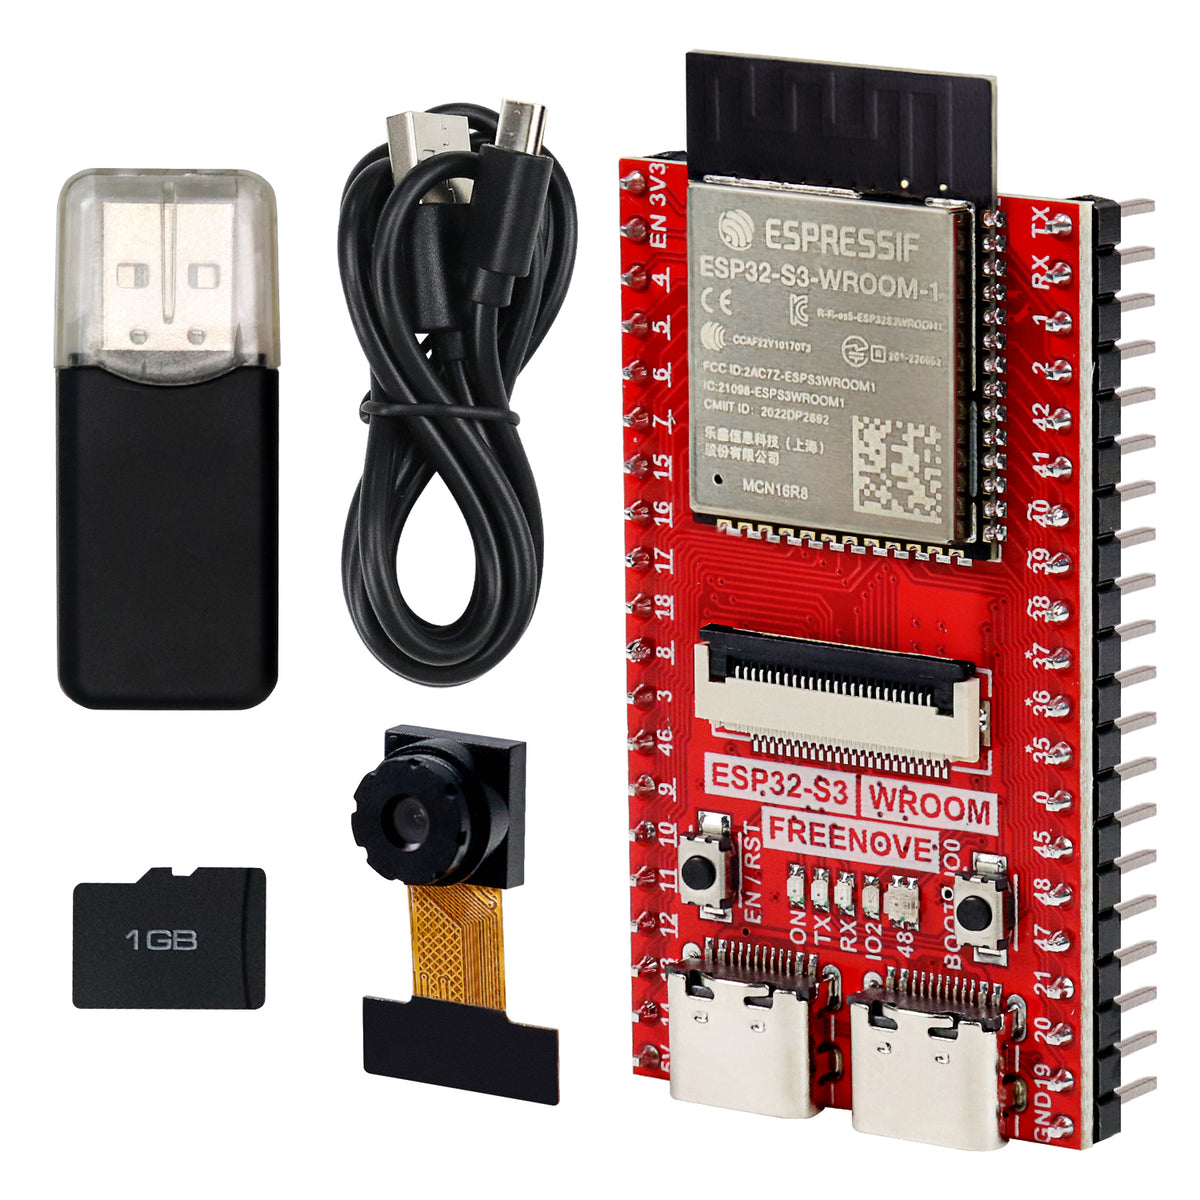
\includegraphics[width=0.22\textwidth,height=2.1cm,keepaspectratio]{../reports_latex/assets/components/esp32s3_freenove.jpg} &
        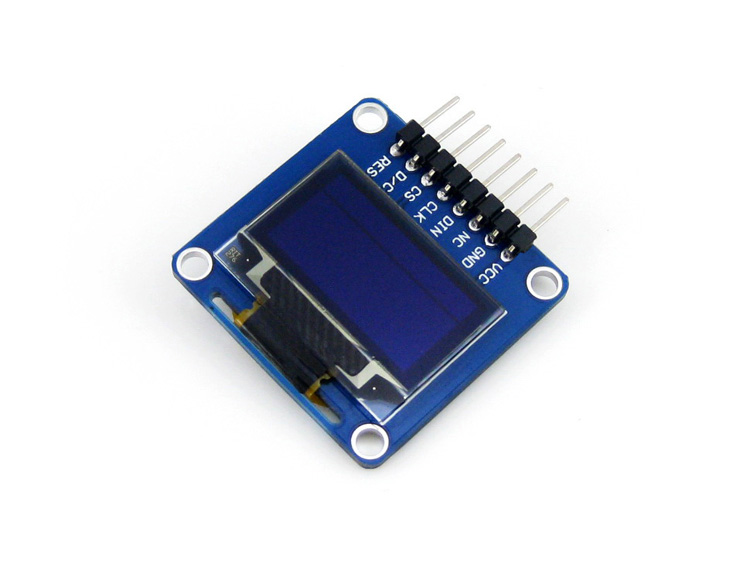
\includegraphics[width=0.22\textwidth,height=2.1cm,keepaspectratio]{../reports_latex/assets/components/oled_ssd1306.jpg}\\[1mm]
        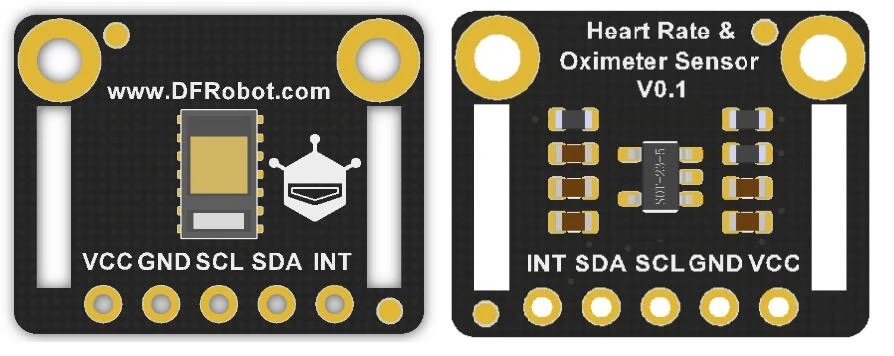
\includegraphics[width=0.22\textwidth,height=1.9cm,keepaspectratio]{../reports_latex/assets/components/max30102_board_overview.jpg} &
        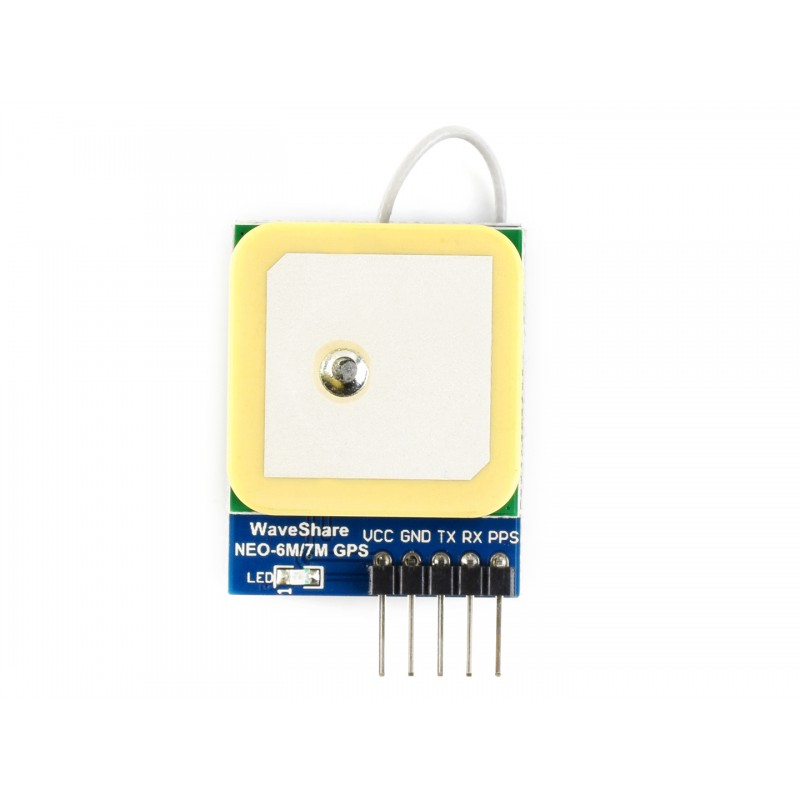
\includegraphics[width=0.22\textwidth,height=1.9cm,keepaspectratio]{../reports_latex/assets/components/gps_neo6m_reference.jpg}
      \end{tabular}
    \end{column}
  \end{columns}
\end{frame}

\begin{frame}{Phạm vi mới: truy cập toàn bộ hệ thống qua Wi-Fi cục bộ}
  \vspace{2mm}
  \begin{columns}[T,onlytextwidth]
    \begin{column}{0.52\textwidth}
      \begin{itemize}\setlength\itemsep{3mm}
        \item ESP32-S3 tự phát mạng, không cần router hay Internet
        \item Captive portal và dashboard responsive cho điện thoại/laptop
        \item API JSON cập nhật mỗi 0,25 giây, không chặn vòng lặp cảm biến
        \item Đặt lại số bước và hủy cảnh báo ngay trên web
      \end{itemize}
    \end{column}
    \begin{column}{0.44\textwidth}
      \fcolorbox{Ink}{Ink}{\parbox{0.92\linewidth}{
        \centering\color{white}\vspace{3mm}
        {\scriptsize\bfseries KẾT NỐI TRONG MẠNG CỤC BỘ}\par\vspace{3mm}
        {\scriptsize\color{LightGray}TÊN WI-FI}\par{\LARGE\bfseries health-monitor}\par\vspace{3mm}
        {\scriptsize\color{LightGray}MẬT KHẨU}\par{\LARGE\bfseries 99999999}\par\vspace{3mm}
        {\scriptsize\color{LightGray}ĐỊA CHỈ}\par{\Large\bfseries 192.168.4.1}\vspace{3mm}}}
    \end{column}
  \end{columns}
\end{frame}

\begin{frame}{ESP32-S3 là trung tâm của kiến trúc}
  \centering
  \begin{tikzpicture}[
    block/.style={draw=Ink,rounded corners=1mm,fill=white,minimum width=30mm,minimum height=10mm,align=center,font=\small},
    core/.style={draw=Ink,very thick,rounded corners=1mm,fill=Ink,text=white,minimum width=40mm,minimum height=15mm,align=center,font=\bfseries},
    arrow/.style={-{Latex[length=2mm]},thick}
  ]
    \node[core] (esp) {ESP32-S3 N16R8\\Lập lịch không chặn};
    \node[block,above left=8mm and 16mm of esp] (ppg) {MAX30102\\RED/IR, FIFO};
    \node[block,left=16mm of esp] (imu) {IMU 0x68\\Gia tốc, số bước};
    \node[block,below left=8mm and 16mm of esp] (gps) {GPS UART\\NMEA 9600};
    \node[block,above right=8mm and 16mm of esp] (algo) {BPM, SpO$_2$\\Chất lượng};
    \node[block,right=16mm of esp] (fall) {Té ngã\\NORMAL--ALERT};
    \node[block,below right=8mm and 16mm of esp] (ui) {OLED/Buzzer\\Cảnh báo};
    \node[block,below=13mm of esp] (web) {Wi-Fi AP + HTTP/DNS tự viết\\Dashboard + JSON API};
    \draw[arrow] (ppg)--(esp); \draw[arrow] (imu)--(esp); \draw[arrow] (gps)--(esp);
    \draw[arrow] (esp)--(algo); \draw[arrow] (esp)--(fall); \draw[arrow] (esp)--(ui); \draw[arrow] (esp)--(web);
  \end{tikzpicture}
  \vspace{2mm}\par\muted{Một nguồn dữ liệu dùng chung cho OLED, Serial và dashboard web.}
\end{frame}

\begin{frame}{Thông số cơ bản được chọn theo đúng cấu hình firmware}
  \scriptsize
  \begin{tabularx}{\textwidth}{>{\bfseries}l l l X}
    \toprule
    Mô-đun & Giao tiếp & Cấu hình đang dùng & Chức năng\\
    \midrule
    ESP32-S3 N16R8 & 240 MHz & Flash 16 MB, PSRAM 8 MB & Điều phối và Wi-Fi AP\\
    OLED SSD1306 & I2C 0x3C & 128$\times$64, cập nhật 10 Hz & Hiển thị tại chỗ\\
    MAX30102 & I2C 0x57 & ADC 18 bit; 400 Hz/4 $\Rightarrow$ 100 Hz & RED/IR, BPM, SpO$_2$\\
    IMU 6 trục & I2C 0x68 & $\pm2g$, DLPF 44 Hz, đọc 50 Hz & Bước và té ngã\\
    GPS NEO-6M/7M & UART1 & 9.600 baud, GGA/RMC & Vị trí và vệ tinh\\
    Buzzer & LEDC PWM & GPIO42; 1,7/2,3 kHz & Cảnh báo xen kẽ\\
    \bottomrule
  \end{tabularx}
  \vspace{3mm}
  \fcolorbox{Ink}{LightGray}{\parbox{0.94\textwidth}{\centering\bfseries GPIO8--9 là bus I2C chung; GPS tách sang RX21/TX47 và buzzer dùng GPIO42.}}
\end{frame}

\begin{frame}{Các driver và thuật toán chính đều do nhóm tự viết}
  \begin{columns}[T,onlytextwidth]
    \begin{column}{0.48\textwidth}
      {\large\bfseries Lớp giao tiếp phần cứng}\par\vspace{2mm}
      \small
      \begin{itemize}\setlength\itemsep{1.8mm}
        \item Đọc/ghi thanh ghi I2C và FIFO MAX30102
        \item Framebuffer, font 5$\times$7 và lệnh SSD1306
        \item Đọc 6 byte gia tốc, PWM buzzer
        \item Gom UART, checksum và parser NMEA
      \end{itemize}
    \end{column}
    \begin{column}{0.49\textwidth}
      {\large\bfseries Lớp xử lý và dịch vụ}\par\vspace{2mm}
      \small
      \begin{itemize}\setlength\itemsep{1.8mm}
        \item IIR, ngưỡng thích nghi, RR và ratio-of-ratios
        \item Bộ đếm bước và máy trạng thái té ngã
        \item DNS wildcard, parser HTTP, router và JSON
        \item Máy trạng thái phục hồi từng cảm biến
      \end{itemize}
    \end{column}
  \end{columns}
  \vspace{3mm}
  \fcolorbox{Ink}{Ink}{\parbox{0.93\textwidth}{\centering\color{white}\small\bfseries Chỉ dùng Arduino Core, Wire, HardwareSerial, WiFi và WiFiUDP làm lớp nền truy cập phần cứng; không dùng thư viện cảm biến hay thuật toán hoàn chỉnh.}}
\end{frame}

\begin{frame}{Vòng lặp không chặn giữ dữ liệu và web hoạt động đồng thời}
  \centering
  \vspace{3mm}
  \begin{tikzpicture}[
    p/.style={draw=Ink,rounded corners=1mm,fill=white,minimum width=31mm,minimum height=14mm,align=center,font=\small},
    a/.style={-{Latex[length=2mm]},thick},node distance=7mm
  ]
    \node[p] (http) {DNS + HTTP\\không chờ};
    \node[p,right=of http] (read) {GPS liên tục\\FIFO PPG};
    \node[p,right=of read,fill=LightGray] (task) {Tác vụ theo mốc\\IMU, OLED, log};
    \node[p,right=of task] (recover) {Kiểm tra lỗi\\và phục hồi};
    \draw[a] (http)--(read); \draw[a] (read)--(task); \draw[a] (task)--(recover);
    \draw[a] (recover.south) -- ++(0,-8mm) -| (http.south);
  \end{tikzpicture}
  \vspace{6mm}\par
  \bigmetric{100 Hz}{PPG}\hfill
  \bigmetric{10 Hz}{OLED}\hfill
  \bigmetric{4 Hz}{Dashboard}
  \vspace{2mm}\par\muted{Ba nhịp thời gian cùng chạy mà không dùng trì hoãn dài.}
\end{frame}

\begin{frame}{PPG tự lọc RED/IR rồi xác nhận BPM theo khoảng RR}
  \centering
  \begin{tikzpicture}[node distance=3mm, b/.style={draw=Ink,rounded corners=1mm,minimum width=23mm,minimum height=9mm,align=center,font=\scriptsize}, a/.style={-{Latex[length=2mm]},thick}]
    \node[b] (a) {FIFO\\100 Hz}; \node[b,right=of a] (b) {Nhận/ngắt\\ngón tay};
    \node[b,right=of b] (c) {Tách DC/AC\\Lọc IIR}; \node[b,right=of c] (d) {Dò nhịp\\Tự nhận cực tính};
    \node[b,right=of d,fill=Ink,text=white] (e) {BPM / SpO$_2$\\Cờ hợp lệ};
    \draw[a](a)--(b);\draw[a](b)--(c);\draw[a](c)--(d);\draw[a](d)--(e);
  \end{tikzpicture}
  \vspace{2mm}
  \begin{columns}[T,onlytextwidth]
    \begin{column}{0.50\textwidth}
      \scriptsize
      \begin{itemize}\setlength\itemsep{0.5mm}
        \item ADC 400 Hz, trung bình 4 mẫu $\Rightarrow$ FIFO 100 Hz
        \item Xung LED 411 $\mu$s, dòng khoảng 10 mA, dải 4.096 nA
        \item Bám nền 350 ms; ngưỡng $0{,}55\times$ đường bao
        \item BPM $=60.000/\Delta t_{RR}$, miền xác nhận 40--180 BPM
      \end{itemize}
    \end{column}
    \begin{column}{0.47\textwidth}
      \scriptsize
      \begin{itemize}\setlength\itemsep{0.5mm}
        \item BPM sơ bộ từ nửa chu kỳ, sau đó thay bằng RR đầy đủ
        \item SpO$_2$: RMS(AC)/DC của RED và IR trong 64 mẫu
        \item Phiên đo mới tự làm sạch MAX30102 và FIFO
        \item Kẹt quá 3,5 s: tự khởi tạo lại, không cần Serial Monitor
      \end{itemize}
    \end{column}
  \end{columns}
  \vspace{0.5mm}\par
  \fcolorbox{Ink}{white}{\parbox{0.91\textwidth}{\centering\small\bfseries SpO$_2$ là giá trị ước lượng nguyên mẫu, chưa hiệu chuẩn bằng thiết bị y tế.}}
\end{frame}

\begin{frame}{IMU phục vụ đếm bước và máy trạng thái té ngã}
  \begin{columns}[T,onlytextwidth]
    \begin{column}{0.47\textwidth}
      {\large\bfseries Đếm bước}\par\vspace{2mm}
      \small
      \begin{itemize}\setlength\itemsep{1.5mm}
        \item IIR tách trọng lực: $\alpha=0{,}03$; lọc động $\alpha=0{,}25$
        \item Xác nhận đáy $<-0{,}05g$ rồi đỉnh $>0{,}11g$
        \item Chu kỳ hợp lệ 280--1.800 ms; tổng gia tốc $<1{,}8g$
        \item Hai đỉnh liên tiếp mới xác nhận chuỗi đi bộ
      \end{itemize}
    \end{column}
    \begin{column}{0.50\textwidth}
      {\large\bfseries Phát hiện té ngã}\par\vspace{1mm}
      \centering
      \flowstate{NORMAL}{Theo dõi}\par$\downarrow$\par
      \flowstate{FREEFALL}{$<0{,}45g$ trong 120 ms}\par$\downarrow$\par
      \flowstate{IMPACT}{$>2{,}2g$; trực tiếp nếu $>2{,}8g$}\par$\downarrow$\par
      \flowstate{ALERT}{Sau 1,8 s: ít chuyển động, 0,72--1,28g}
      \vspace{1mm}\par\tiny\muted{Không đủ điều kiện trong 5 s: quay về NORMAL.}
    \end{column}
  \end{columns}
\end{frame}

\begin{frame}[fragile]{GPS chỉ nhận câu NMEA vượt qua checksum}
  \begin{columns}[T,onlytextwidth]
    \begin{column}{0.43\textwidth}
      \vspace{1mm}
      {\large\bfseries WAIT $\rightarrow$ NOFIX $\rightarrow$ FIX}\par
      \vspace{2mm}
      \small
      \begin{itemize}\setlength\itemsep{1.2mm}
        \item UART có byte nhưng chưa đủ vệ tinh: NOFIX, không phải mất GPS
        \item GGA: chất lượng fix, vệ tinh, tọa độ; RMC: trạng thái A/V
        \item LOST khi UART ngừng quá 3 giây
        \item Tọa độ hợp lệ gần nhất được giữ riêng
        \item Dashboard chỉ mở bản đồ khi parser đã xác nhận vị trí
      \end{itemize}
    \end{column}
    \begin{column}{0.53\textwidth}
\begin{lstlisting}[style=slidecode]
(*@\textcolor{CodeComment}{\sffamily\itshape // Tính XOR phần thân câu NMEA.}@*)
uint8_t checksum = 0;
for (const char *p = sentence + 1;
     p < star; p++) {
  checksum ^= (uint8_t)*p;
}
return checksum == expected;
\end{lstlisting}
      \vspace{1mm}\par\centering\small\bfseries Câu sai checksum bị loại trước khi parser tách trường.
    \end{column}
  \end{columns}
\end{frame}

\begin{frame}{Dashboard hiển thị toàn bộ trạng thái trên một màn hình}
  \centering
  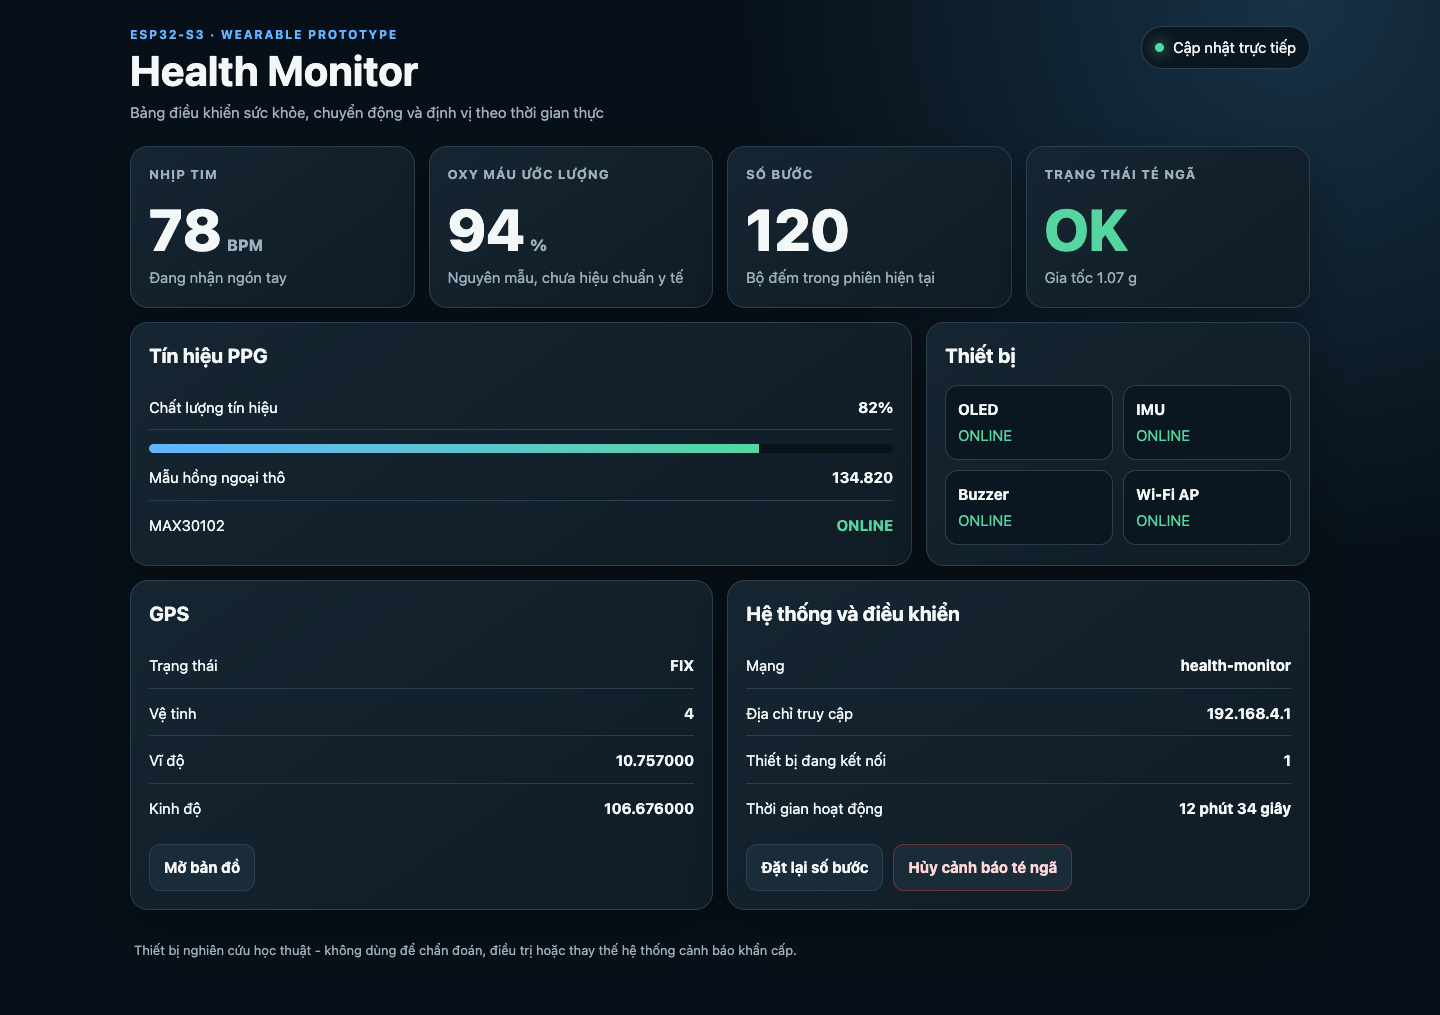
\includegraphics[width=0.90\textwidth,height=5.25cm,keepaspectratio]{../reports_latex/assets/web/dashboard_preview.png}
  \vspace{-1mm}\par\tiny\muted{Bản render dùng dữ liệu minh họa; khi chạy thật, giao diện lấy JSON từ ESP32-S3 mỗi 0,25 giây.}
\end{frame}

\begin{frame}{Luồng dữ liệu từ cảm biến đến dashboard}
  \begin{columns}[T,onlytextwidth]
    \begin{column}{0.48\textwidth}
      {\Large\bfseries Luồng cập nhật}\par\vspace{3mm}
      \small
      \begin{enumerate}\setlength\itemsep{1.5mm}
        \item Firmware cập nhật trạng thái dùng chung
        \item \texttt{/api/status} tạo JSON khi có yêu cầu
        \item JavaScript cập nhật thẻ số đo mỗi 0,25 giây
        \item POST đặt lại bước hoặc hủy ALERT
      \end{enumerate}
    \end{column}
    \begin{column}{0.48\textwidth}
      {\Large\bfseries Trường hiển thị}\par\vspace{3mm}
      \small
      \begin{tabularx}{\linewidth}{>{\bfseries}l X}
        PPG & BPM, SpO$_2$, chất lượng, RED/IR\\
        IMU & bước, gia tốc, chuyển động, té ngã\\
        GPS & trạng thái, vệ tinh, tọa độ, byte\\
        Thiết bị & OLED, IMU, MAX30102, buzzer\\
        Hệ thống & uptime, số máy khách, IP\\
      \end{tabularx}
    \end{column}
  \end{columns}
  \vspace{1mm}\par
  \fcolorbox{Ink}{Ink}{\parbox{0.92\textwidth}{\centering\color{white}\small\bfseries Một ESP32-S3 duy trì PPG 100 Hz và dashboard 4 Hz; HTTP, DNS, JSON cùng toàn bộ giao diện đều do nhóm tự viết và lưu trong flash.}}
\end{frame}

\end{document}
